%#########################################################################################
\chapter{Evaluation}
\label{chap:evaluation}
%#########################################################################################

In the previous chapter, STODaP approach was presented in details, as well as the supporting tools and their implementation choices.
Practical results were also characterized, showing concrete achievements on the open data organization problem.

In this chapter, the evaluation of STODaP server is described.
The system was compared to other mechanisms on the task of searching for open datasets.
We first present a theoretical background on search engine evaluation methodologies in \autoref{sec:lit_review}.
Then, we show the experimental setup in \autoref{sec:setup}, the pre-evaluation procedure in \autoref{sec:pre_evaluation} and the results in \autoref{sec:eval_results}.
Some concluding remarks are driven on the final section.

\section{Methodology Background}
\label{sec:lit_review}

As the amount of online available data gets bigger and bigger, search methodologies are increasingly necessary to allow users accessing relevant content.
Thus, it is crucial to develop evaluation techniques that allows researchers to compare different algorithms and find the most adequate ones for each context.

\citeonline{Cheng2010} developed two measures for assessing \emph{user satisfaction} and \emph{user effectiveness} on Interactive Information Retrieval systems.
The first one is called Normalized Task Completion Time (NT), and is calculated as the relation between task completion times for novices and experts.
Following the same reasoning, the Normalized User Effectiveness (NUE) evaluates the relation between relevant documents retrieved by novices and experts, proportional to NT.
Authors claim that this normalization procedure turns the measures more stable against task complexity variations.
Results show that the NT is highly correlated to user satisfaction, while NUE is a better indicator for effectiveness when compared to simple task completion time.
The learning curve was also better explained by NT and NUE than by task completion time.

In a contrary direction, \citeonline{Xu2009} defend the use of task completion time as a robust measure to assess in which extent the search engine helps users to complete a task.
Additionally, these authors found a negative correlation between user satisfaction and task completion time.
An important result of this study is a mathematical development which shows that a cross-over design reduces significantly the variance of the experiment.
Cross-over design means that, when comparing systems A and B on several tasks, every user tests both systems and completes all tasks once, half of them in A, and the other half in B.
For tasks T1 and T2, we would have half of the users performing performing T1 with method A and T2 with method B, and half of them performing T1-B and T2-A.

%config 1: metade dos usuarios usam um sistema, metade outro, todos fazem todas as tarefas
%config 2: todos fazem todas as tarefas nos dois sistemas > problema : curva de aprendizado - solução - crossover - todos usuarios vao usar os dois sistemas, mas para tarefas diferentes : metade dos usuarios faz metade das tarefas no A e metade no B, e vice-versa

In a survey dealing specifically with faceted search, \citeonline{Wei2013} presents a review about relevance and cost-based metrics on the faceted search context.
Regarding relevance metrics, authors go through a number of works which use precision, recall or F-measure in the same way as on non-faceted search evaluation.
Cost-based metrics look at the time needed to complete a search task, and memory usage.
These metrics were used to compare performance between faceted and non-faceted engines.

Although the Web and search engines have dramatically changed in the last 10 years, the perspective brought by \citeonline{Vaughan2004} is still relevant.
The focus in this work relies on the quality of ranking, i.e., the order in which results are presented.
Both works presented previously rely on the task completion time, which brings with it factors that do not depend on the system, e.g., users ability, and factors not directly related to the search-engine, such as usability.
By looking specifically at the ranking quality, the evaluation methodology may ignore these aspects, and keeps full attention on the search mechanism.
In this work, author proposes non-binary counterparts to the traditional precision and recall measures, with the intention of adding human relevance judgement aspects to the evaluation.
Specifically, two measures are proposed: (i) \emph{Quality of result ranking}, as counterpart of precision and (ii) \emph{Ability to retrieve top ranked pages}, as counterpart measure of recall.
Both measures rely on a human driven ranking of results, which is correlated with the search engine one in the first case.
The second measure evaluates in which extent the top-results are present in each search engine, for the same query.

\section{Experimental Setup}
\label{sec:setup}

% -- hiposteses e metricas

% \citeonline{Cheng2010}
% entry questionaire to make sure the users were able to make the test
% novices received a basic training, reading instructions and questions we answered
% The researchers ran a pilot study before finalizing the search tasks to make sure that LexisNexis Academic could retrieve the relevant documents for all these search tasks. Each
% For each search task, the subject stopped the search session when either the information need was satisfied or he or she gave up the task. The researchers observed the subjects performing their searches in order to ensure that the correct procedures were being followed. The researchers also recorded the task completion time of each task, and asked the subjects to answer a questionnaire after each task. As
% 4. Task completion time (T): The time from the start until the completion of a retrieval task. The task completion time is recorded in seconds, but note that the minute was the unit in the calculations. The subjects stopped each search session by themselves, either once their search needs were satisfied or when they gave up.
% 5. User satisfaction (S): An ordinal number indicating the level of user satisfaction. A questionnaire was provided to the users after each search was complete. It asked the subjects to rate their satisfaction level towards the system in regard to supporting the accomplishment of the search task, using a scale from 1 (not satisfied at all) to 5 (extremely satisfied).

In this section, we describe in details our experimental setup.

\subsection{Goals and Metrics} % (fold)

First of all, we define the evaluation goals:
\begin{itemize}
	\item G1: When searching for open data, how does STODaP compares to other data-specific and general search engines?
	\item G2: Is the STODaP server an useful tool for searching open datasets?
\end{itemize}

G1 will be answered through objective assessments.
Metrics in this case will be: 

\noindent \textbf{Task Completion Time (TCT)}: the amount of seconds that a subject takes to finish a task, i.e., answering a question using a specific searching method.
A task is finished when the subject clicks the ``Finish'' button, and the evaluation framework will automatically calculate TCT.
Subject validation methods will be used to guarantee that tasks not performed adequately are not considered as valid.
Normalized TCT, as proposed by \citeonline{Cheng2010}, was also considered. 
However, the structure to guarantee a reasonable number of experts was not available.

\noindent \textbf{Precision}: As detailed bellow, each question requires subjects to find $N$ datasets according to a defined specification.
Thus, we define Precision as the number of true positives, i.e., answered datasets truly corresponding to the question definition, divided by the sum of true positives and false positives, i.e., $N$.
In this case, calculating a recall measure is not viable, since the definition of questions is broad enough to make the calculation of all true possibilities nearly impossible.


The second goal (G2) relies on subjective evaluation of users.
In this case, metrics are defined by a questionnaire presented after the evaluation, and contains both a question about absolute user satisfaction, and another related to satisfaction in relation to other methods.
In order to compare STODaP performance, we selected two other search methods:

\begin{itemize}
	\item \textbf{Exversion: } Exversion Data Search Engine\footnote{Available at \url{https://www.exversion.com/search/}} is similar to STODaP because it indexes open datasets from ODPs and provides a unified search interface.
	However, no semantics is applied.
	\item \textbf{Free: } As observed in \autoref{sec:obs_based_analysis}, the first impulse of users search for open dataset is to use generic web search engines such as Google, DuckDuckGo, Yahoo, and others.
	Thus, we included a free search to let users choose their preferred search engine.
\end{itemize}

\subsection{Subjects}

The aim of STODaP server is to facilitate access to open data to the general public.
We consider that experts already have their own strategies and sources for finding adequate data.
Thus, we do not require experience in open data.
However, users must have some previous knowledge on internet navigation. 
Knowledge on basic data processing tools such as spreadsheet processors is also desired, so that subjects can at least imagine a potential use of data.
English knowledge is also necessary, because labels of semantic tags and groups are still only in English language.


\subsection{Tasks}

By design, STODaP server is a tool for interlinking different Open Data Portals.
Thus, in this evaluation we aim to assess the ability of gathering similar information from several ODPs, rather than finding specific datasets on the Web.

The evaluation questions where selected based on: (i) topic relevance of datasets on the open data community, based on criteria defined by Open Data Index\footnote{http://index.okfn.org/} (ii) the existence of search results on STODaP server.
This restriction allows us only to make assertions about the performance of STODaP server on the topics covered by the system, which consists of large base of open data portals, as described in \autoref{sec:stodap_architecture}.
Broader conclusion would require evaluations of larger scales, which are over the scope of this thesis.
Defined questions are:

\begin{itemize}
	\item \textbf{Q1}: Find open datasets about \textbf{water quality} on \textbf{7 different rivers}.
	\item \textbf{Q2}: Find open datasets containing \textbf{2015 budget data} from locations in \textbf{5 different countries}.
	\item \textbf{Q3}: Find open datasets containing \textbf{procurement information} in \textbf{3 different languages}.
\end{itemize}

\subsection{Procedure}

The following procedure was driven during the evaluation process:

\begin{itemize}
	\item The main idea of the project is explained, followed by an explanation about the evaluation itself;
	\item Participants fill the entry-questionnaire, shown in \autoref{tab:entry_questionnaire}; 
	\item After finishing the form, three tasks are sequentially presented. 
	Each task is a combination of a question Q and a search method M.
	Combinations for each participant are chosen in order to guarantee that each Q-M combination has approximately the same number of answers.
	\item For each task, the appropriate number of text fields are presented for pasting the dataset links.
	\item The time taken to complete each task is automatically calculated.
	\item The evaluation questionnaire shown in \autoref{tab:eval_questionnaire} is presented to the subjects.
\end{itemize}

\begin{table}[h]
\ABNTEXfontereduzida
\centering
\caption[Entry questionnaire.]{Entry questionnaire.}
\label{tab:entry_questionnaire}
\begin{tabular}{|>{\arraybackslash}m{3cm}|>{\arraybackslash}m{7cm}|>{\arraybackslash}m{5cm}|}
\hline
\centering\textbf{ID} & \centering\textbf{Question} & \centering\arraybackslash\textbf{Range} \\ \hline
Age & How old are you?  & $> 0$ \\
Internet & How often do you use internet? & 1 - once a week; 5 - everyday \\
Data & How often do you use structured data in your study/work? (e.g. spreadsheets, charts, statistics, ...) & 1 - never; 5 - always \\
Open Data & How often do you use open data in your study/work? & 1 - never; 5 - always \\
English & What is your English proficiency level? & 1 - low ; 5 - high \\
\hline
\end{tabular}
\end{table}

\begin{table}[h]
\ABNTEXfontereduzida
\centering
\caption[Evaluation questionnaire.]{Evaluation questionnaire.}
\label{tab:eval_questionnaire}
\begin{tabular}{|>{\arraybackslash}m{3cm}|>{\arraybackslash}m{7cm}|>{\arraybackslash}m{5cm}|}
\hline
\centering\textbf{ID} & \centering\textbf{Question} & \centering\arraybackslash\textbf{Range} \\ \hline
Absolute Satisfaction & Do you think STODaP is a useful tool for finding data on the web? & 1 - not useful; 5 - very useful \\
Relative Satisfaction & How easy is it was get the data you need using the STODaP in comparison with the other methods? & 1 - harder; 5 - easier \\
Comments & If you have additional comments or suggestions, please write it here: & Free text \\
\hline
\end{tabular}
\end{table}

\subsection{Validation}
Each entry-questionnaire was analysed in order to determine if it is valid to our evaluation, in terms of internet experience.
Subjects are only validated if they complete all tasks and the evaluation questionnaire.

Individual answers are checked in order to confirm if the dataset links provided are really valid answers according to the assigned question.


%#######################################
\section{Pre-Evaluation}
\label{sec:pre_evaluation}
%#######################################

In order to test and adjust our evaluation setup, we ran the process described above with a group of seven students of an Information Retrieval graduate course, at the Federal University of Rio de Janeiro, on the 12th of May 2016.
The results of this evaluation round can be seen in \autoref{tab:pre_eval_questionnaire} and \autoref{tab:pre_eval_results}.
Although the main target of this pre-evaluation process was to assess the evaluation procedure (and not the STODaP server), it is useful to look at the results to have the first impressions.

\begin{table}[h]
\ABNTEXfontereduzida
\centering
\caption[Answers to the entry and evaluations questionnaires.]{Answers to the entry and evaluations questionnaires. Columns correspond to the entry-questionnaire, applied before the evaluation, and the evaluation one, filled afterwards. Full question text can be seen in \autoref{tab:entry_questionnaire} and \autoref{tab:eval_questionnaire}. Task Completion Time (TCT) is the average number of seconds taken to finish the task. Precision is the percentage of answers considered valid, over a total of 15.}
\label{tab:pre_eval_questionnaire}
\begin{tabular}{|>{\centering\arraybackslash}m{.5cm}|>{\centering\arraybackslash}m{.7cm}|>{\centering\arraybackslash}m{1.cm}|>{\centering\arraybackslash}m{.8cm}|>{\centering\arraybackslash}m{.8cm}|>{\centering\arraybackslash}m{2cm}|>{\centering\arraybackslash}m{2.4cm}|>{\centering\arraybackslash}m{2.4cm}|>{\centering\arraybackslash}m{1.3cm}|}
\hline
& 	Age & Internet & Data  & Open Data &	Absolute Satisfaction &	Relative Satisfaction &  TCT & Precision (\%)\\ \hline
1& 	27& 	5& 	3& 	1& 	4& 	2& 	295.7 +/- 98.8 & 100 \\ \hline
2& 	23& 	5& 	4& 	3& 	5& 	3& 	833.3 +/- 151.8 & 80 \\ \hline
3& 	27& 	5& 	5& 	5& 	2& 	2& 	560.0 +/- 103.2 & 33 \\ \hline
4& 	23& 	5& 	4& 	3& 	5& 	4& 	845.0 +/- 523.9 & 73 \\ \hline
5&	26& 	5& 	3& 	2& 	5& 	5& 	625.3 +/- 269.5 & 67 \\ \hline
6& 	29& 	5& 	5& 	3& 	4& 	4& 	527.0 +/- 287.5 & 100 \\ \hline
7& 	22& 	5& 	4& 	1& 	5& 	5& 	351.0 +/- 121.2 & 80 \\ \hline
\end{tabular}
\end{table}

\begin{table}[]
\ABNTEXfontereduzida
\centering
\caption[Task Completion Time of the pre-evaluation test, in seconds.]{Task Completion Time of the pre-evaluation test, in seconds. 
Each cell contains the number of seconds that one or more subjects took to complete the task with the correspondent search method.}
\label{tab:pre_eval_results}
\begin{tabular}{|>{\centering\arraybackslash}m{2.0cm}|>{\centering\arraybackslash}m{2.4cm}|>{\centering\arraybackslash}m{2.4cm}|>{\centering\arraybackslash}m{2.4cm}|>{\centering\arraybackslash}m{2.4cm}|>{\centering\arraybackslash}m{2.0cm}|}
\hline
\textbf{Questions / Search Methods} & \textbf{Q1: Water Quality} & 	\textbf{Q2: Budget information} &	\textbf{Q3: Procurement} &	\textbf{Average and Standard Deviation} & \textbf{Accepted Answers (\%)} \\ \hline
\textbf{Exversion} &	723, 884, 468 &	235, 382 &	558, 518 &	538.3 +/- 198.5 & 78 \\ \hline
\textbf{STODaP} &	435, 493, 460 &	397, 184, 517, 1048 & -	&	504.9 +/- 244.0 & 83 \\ \hline
\textbf{Free} &	1580 &	702 &	401, 217, 180, 1001, 729 &	687.1 +/- 456.3 & 63 \\ \hline
\textbf{Average and Standard Deviation} &	720.4 +/- 383.7 &	495.0 +/- 276.7 &	514.9 +/- 266.7 & & \\ \hline
\textbf{Accepted Answers (\%)} & 76 & 80 & 71 & & \\ \hline
\end{tabular}
\end{table}

\autoref{tab:pre_eval_questionnaire} shows the answers of each subject to the questions both before and after running the evaluation, together with its average task completion time and precision.
As expected, all subjects are frequent internet users.
Use of data in daily work or study is also high, but the only one declared himself an open data expert.
Coincidently or not, this subject was the only who did not considered STOaP an useful tool for finding data on the web.
Four out of seven considered that completing the tasks with STODaP was easier than with other methods.
The average Task Completion Time had a huge variation, with a minimum of 295 seconds and a maximum of 845 seconds.
Through a manual procedure, each answer was verified in order to check if it really corresponds to the given task.
The verification was not strict, and answers were discarded only if they were clearly wrong, or blank.
No significant correlation was verified between TCT and precision.

\autoref{tab:pre_eval_results} shows the Task Completion Times for each task.
We can easily notice that a choosing a random generator for attributing question / search methods combination was a mistake, specially with a small number of rounds.
There were 36 possibilities (6 orderings for questions $\times$ 6 orderings for search methods) but only 7 rounds were used.
Thus, the number of combinations between questions and search methods ended up quite unbalanced, and there was no combination of STODaP search method with the procurement task.
Average TCT for tasks and search methods were also calculated.

After running the procedure, a conversation round was driven with the students on order to get insights both about the tool and the evaluation procedure.
The following suggestions and comments were made:

Regarding the evaluations interface:

\begin{itemize}
	\item Alert that search engines should be opened in another tab;
	\item Write the questions more clearly and specific (e.g., asking budget 2015 may include 2014-16?)
	\item On the final questions, positive answers to the system were at the left side, which is not usual and confused some subjects;
	\item State more clearly that only the link to the dataset should be answered;
	\item Makes clear that users are allowed to use auxiliary tools such as translators or Wikipedia in order to better perform the tasks;
	\item State more clearly that users should only look to the dataset title, and there is no need to open it;
	\item Explain that only some specific portals are indexed, not all open data in the world.
\end{itemize}

Regarding the evaluations procedure:
\begin{itemize}
	\item On the evaluation questionnaire, ask the English proficiency and other languages, and ask if the English language hampered the performance;
	\item There were to few questions, and thus learning curve was not evaluated.
\end{itemize}
	
Regarding the STODaP faceted search interface:
\begin{itemize}
	\item There should be an explanation about faceted search and how does it work;
	\item Regarding the Portal facets, it was suggested to write portals name in spite of URLs, when this metadata is available
	\item One participant reported that he took a while to realize the language facet; after seeing it, question Q3 could be very quickly answered.
	\item It was suggested to include the possibility of making the query broader by including facets with OR.
\end{itemize}	

There were some positive comments:
\begin{itemize}
	\item It was noted that results presented by STODaP had a higher quality in relation to Exversion, mainly because the latter automatically uses an OR logic between two terms.
	This results in many unwanted outputs.
	\item The possibility of searching English keywords and getting multi-language results was also positively mentioned, because no other tool presents such feature.
	\item The STODaP interface, in its search results, exhibits datasets with all its tags.
	This was positively noted, because it helps to decide quicker if a dataset is of interest or not.
\end{itemize}	

Analysing students while they were completing their tasks was also show some new perspectives.
It was noticed that some subjects tried to look deep at datasets in order to verify if they met the task criteria.
It should be harder stressed in the explanation that this is not necessary, since the our objective is only to find dataset, and not to verify their quality.
Some students tried to use analytic tools such as Google Public Data.
Their focus is rather on analysing (open) data sets than on making them available for download in machine readable formats.
Thus, for our intentions, this is not considered open data and it should also be stated in the explanation.

After considering the above mentioned comments, the procedure was enhanced and applied to the main groups.
Results are described bellow.

%###############################################################
\section{Results}
\label{sec:eval_results}
%###############################################################

In this section, we describe the application of the evaluation procedure and present the results achieved.

\subsection{Subjects Profile}

Three rounds of the experiment were run.
In the first round, participants were first year university students attending a class on the topic Introduction to Information Systems, at the Federal University of Rio de Janeiro, in Brazil.
The second and third round were online, being one with Semantic Web researchers in Bonn (Germany) and Rio de Janeiro (Brazil), and another within a discussion group of open data practitioners in Brazil.
An entry-questionnaire was filled by the participants, whose answers are summarized in \autoref{tab:eval_summary}.
Participation was not mandatory and non identified, and there was no reward for participants.

\begin{table}[b]
\ABNTEXfontereduzida
\centering
\caption{STODaP evaluation - summary of subjects profile}
\label{tab:eval_summary}
\begin{tabular}{|p{4cm}|>{\centering\arraybackslash}m{2cm}|}
\hline
\textbf{Question} & \textbf{Average} ($n=34$) \\ \hline
Age & 25.7 \\ \hline
Internet & 5\\ \hline
Data & 3.3\\ \hline
Open Data & 2.7 \\ \hline
English & 4.3\\ \hline
\end{tabular}
\end{table}

The average age of the 37 participants was 25.9 years.
Although all of them use internet every day, direct experience with data processing is mid-low, as well as with open data.
As our tool is developed for non-experts, this sample is adequate to the experiment.

After filling the entry questionnaire, subjects were presented 3 combinations of tasks and search methods.
Subjects were instructed to find the specified datasets and paste their URLs in the appropriated fields. The task completion time was automatically calculated for every task of every subject, and correctness of each dataset regarding the specified task was manually checked.
A screenshot of the evaluation tool is shown in \autoref{fig:eval_screenshot}. 

\begin{figure}[h!]
\begin{center}
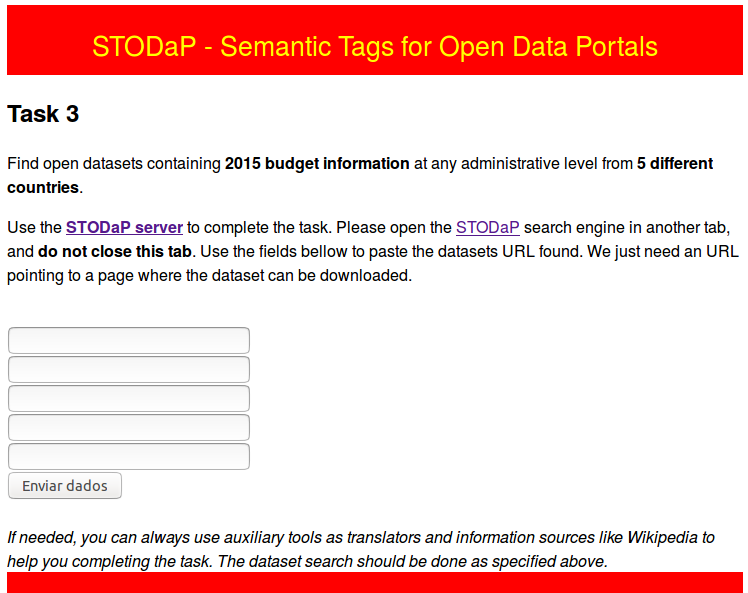
\includegraphics[width=\columnwidth]{images/eval_screenshot.png}
\caption[Evaluation]{Evaluation}
\label{fig:eval_screenshot}
\end{center}
\end{figure}

\subsection{Task Completion Time Analysis}

As detailed above, TCT analysis evaluates the time each subject takes to complete a task.
Although it may look simple to assess this metric, some practical questions arose while analysing data.
First of all, the three questions defined for this evaluation required a different number of datasets to be found.
Thus, because only the total time $T$ for each task is calculated, we divide $T$ by the number $N$ of required datasets to achieve TCT. Thus:

\begin{equation}
	\textrm{TCT} = \frac{T}{N},
\end{equation}
where $T$ is the amount of seconds a subject takes to finish a task, and $N$ is the number of datasets required be each task.

In order to remove disturbing samples, we considered only answers with precision higher than 33\% and TCT lower than 1000 seconds.
The first case is aimed to remove subjects who gave up without trying to complete the task, or who did not understand the task.
Regarding the second case, since some evaluations were made online, we considered that subjects who took more than 1000 seconds to find a dataset actually gave up and left the evaluation tool open.

Another issue is related to the computation of wrong and blank answers.
If a subject answers a question with a dataset that do not correspond to what was asked, there are two options: either an effort was taken, but the question was misunderstood, or no effort was taken at all and a random answer was given\footnote{In order to illustrate this case, one user answered ``www.google.com'' when asked for procurement datasets.}.
The same reasoning applies to blank answers, but in this case the probability that no effort was taken looks higher.
After these considerations, the issue remains: if a question requires 7 datasets, and 3 were correctly answered and 4 were left blank (or were wrong), is it fair to divide $T$ by $N=7$? Or should we divide it by 3, considering that effort was put only on those answers?

In order to evaluate the impact of these considerations, we define:

\begin{equation}
	\textrm{TCT}_{nb} = \frac{T}{N_{nb}},
\end{equation}
where $T$ is the amount of seconds a subject takes to finish a task, and $N_{nb} \leq N$ is the number of not blank answers, and 

\begin{equation}
	\textrm{TCT}_{c} = \frac{T}{N_c},
\end{equation}
where $T$ is the amount of seconds a subject takes to finish a task, and $N_c \leq N$ is the number of datasets correctly answered.
Note that TCT $\leq$ TCT$_{nb} \leq $ TCT$_{c}$.
\autoref{tab:results_TCT}, \autoref{tab:results_TCT_nb} and \autoref{tab:results_TCT_c} present the results for TCT, TCT$_{nb}$ and TCT$_{c}$, respectively.

\begin{table}[h]
\ABNTEXfontereduzida
\centering
\caption[Evaluation Results - TCT.]{Evaluation Results - TCT. Table presents TCT median and standard deviation for each method and question. In brackets, the number of considered samples.}
\label{tab:results_TCT}
\begin{tabular}{|>{\bfseries}c|c|c|c|c|}
\hline
 	& \bfseries{Q1: Water Quality} 	& \bfseries{Q2: Budget} 	& \bfseries{Q3: Procurement} 	& \bfseries{Aggregate} \\ \hline
Exversion 	& 108 $\pm$ 92 (63) 	& 121 $\pm$ 94 (65) 	& 78 $\pm$ 72 (33) 	& 108 $\pm$ 87 (161) \\ \hline
STODaP 	& 60 $\pm$ 49 (77) 	& 63 $\pm$ 170 (50) 	& 67 $\pm$ 80 (42) 	& 60 $\pm$ 109 (169) \\ \hline
Free 	& 60 $\pm$ 126 (70) 	& 44 $\pm$ 37 (50) 	& 100 $\pm$ 96 (24) 	& 70 $\pm$ 99 (144) \\ \hline
Aggregate & 68 $\pm$ 95 (210) 	& 60 $\pm$ 117 (165) 	& 78 $\pm$ 84 (99) 	& \\ \hline 
\end{tabular}
\end{table}

\begin{table}[h]
\ABNTEXfontereduzida
\centering
\caption[Evaluation Results - TCT$_{nb}$.]{Evaluation Results - TCT$_{nb}$. Table presents TCT$_{nb}$ median and standard deviation for each method and question. In brackets, the number of considered samples.}
\label{tab:results_TCT_nb}
\begin{tabular}{|>{\bfseries}c|c|c|c|c|}
\hline
 	& \bfseries{Q1: Water Quality} 	& \bfseries{Q2: Budget} 	& \bfseries{Q3: Procurement} 	& \bfseries{Aggregate} \\ \hline
Exversion 	& 127 $\pm$ 112 (52) 	& 153 $\pm$ 120 (56) 	& 111 $\pm$ 128 (28) 	& 136 $\pm$ 121 (136) \\ \hline
STODaP 	& 60 $\pm$ 49 (77) 	& 63 $\pm$ 170 (49) 	& 67 $\pm$ 80 (42) 	& 60 $\pm$ 109 (168) \\ \hline
Free 	& 64 $\pm$ 146 (62) 	& 44 $\pm$ 37 (50) 	& 100 $\pm$ 96 (24) 	& 70 $\pm$ 109 (136) \\ \hline
Aggregate 	& 74 $\pm$ 114 (191) 	& 60 $\pm$ 129 (155) 	& 83 $\pm$ 107 (94) 	& \\ \hline 
\end{tabular}
\end{table}

\begin{table}[h]
\ABNTEXfontereduzida
\centering
\caption[Evaluation Results - TCT$_{c}$.]{Evaluation Results - TCT$_{c}$. Table presents TCT$_{c}$ median and standard deviation for each method and question. In brackets, the number of considered samples.}
\label{tab:results_TCT_c}
\begin{tabular}{|>{\bfseries}c|c|c|c|c|}
\hline
 	& \bfseries{Q1: Water Quality} 	& \bfseries{Q2: Budget} 	& \bfseries{Q3: Procurement} 	& \bfseries{Aggregate} \\ \hline
Exversion 	& 127 $\pm$ 112 (51) 	& 153 $\pm$ 120 (55) 	& 166 $\pm$ 126 (24) 	& 141 $\pm$ 121 (130) \\ \hline
STODaP 	& 60 $\pm$ 54 (75) 	& 86 $\pm$ 168 (44) 	& 67 $\pm$ 80 (42) 	& 65 $\pm$ 110 (161) \\ \hline
Free 	& 69 $\pm$ 146 (58) 	& 55 $\pm$ 49 (43) 	& 110 $\pm$ 339 (20) 	& 87 $\pm$ 215 (121) \\ \hline
Aggregate 	& 74 $\pm$ 114 (184) 	& 89 $\pm$ 127 (142) 	& 85 $\pm$ 200 (86) 	& \\ \hline 
\end{tabular}
\end{table}

\autoref{tab:results_TCT} shows the general results for TCT.
On each cell, values represent the median, standard deviation and the number of samples in brackets.
Columns represent the different questions, and rows, the search methods.
The last row presents the aggregate results for questions, and the last column, for search methods.
STODaP presents the lowest aggregate TCT median (60 s), followed by free search (70 s, or 17\% higher) and Exversion (108 s, or 80\% higher).
Looking at each question individually, it can be seen that for Q2 (Budget data), free search was faster than STODaP, and for Q1 both were equivalent.
A possible explanation for the budget case is the high availability of this kind of data over the web.
As shortly explained in \autoref{sec:openbudget}, and in details in \citeonline{Tygel2016}, releasing budget data is of crucial importance, and this topic is being prioritized by most of the countries.
Thus, the high availability enables web search engines to deliver faster and more accurate results.

Regarding Q2, a possible explanation can be found on \autoref{tab:results_TCT_nb} and \autoref{tab:results_TCT_c}.
Since Q2 required 7 answers, for this question there was a higher rate of blank answers both on Exversion and free search methods.
Thus, it can be seen in the first column of \autoref{tab:results_TCT_nb} that, while STODaP remains with the same value as in the previous table, the other search methods increase their TCT$_{nb}$ because in those cases, $N_{nb} < N$.
Interestingly, free search presented blank answers only for Q1.
Q2 and Q3 have the same values in \autoref{tab:results_TCT} and \autoref{tab:results_TCT_nb}.
The aggregate result also remained the same.

\autoref{tab:results_TCT_c} presents results related to $TCT_c$.
In this case, STODaP advantage is even higher related free search (34\% higher) and Exversion (117\% higher).
However, in this scenario free search is still faster for Q2.
Results in this table are strongly related to the precision of the answers, which is discussed in the following section.

A last aspect must also be taken into account: standard deviation.
As calculated here, this measure represents the average deviation of each value from the mean value.
If we look to the standard deviations on the tables, it is possible to see that they are very close to the median, and in some cases even higher.
Thus, we look at the TCT for STODaP/Q2 (\autoref{tab:results_TCT}), one could interpret as: ``When using STODaP to answer Q2, users usually take between -107 and 233 seconds to retrieve one dataset''.
This obviously does not make sense.
The two conclusions we can take are: (i) distribution are skewed, i.e., tails are not symmetric around the mean; and (ii) there might be outliers disturbing the standard deviation.
Thus, we show in \autoref{fig:tct}, \autoref{fig:tct_nb} and \autoref{fig:tct_c} the boxplot of TCT, TCT$_{nb}$ and TCT$_c$, respectively.

Boxplot pictures a more detailed view of a distribution, and is specially useful for skewed samples.
Besides the median, marked with a red line in the centre of the box, \autoref{fig:tct} also shows the first and third quartiles, which are the lower and upper bounds of the box.
They represent, respectively, the higher among the one quarter smaller samples, and the smaller among the one quarter higher samples.
Thus, half of the samples are inside the box, whose size is called interquartile range (IQR).
Boxplot shows also outliers: if the distance from an outlier to the median is between 1.5 and 3 IQR, it is pointed with a circle (o); if it is higher than IQR, it is marked with a plus (+).

\autoref{fig:tct} shows that, although STODaP median is lower, IQR is almost at the same position.
Free search lower bound is slightly smaller.
STODaP presented higher outliers, while in Exversion outliers are less disperse.
Moving to \autoref{fig:tct_nb}, where blank answers are not considered, STODaP keeps the lower median, and the lower bound in this case is smaller, meaning that 50\% of the samples are located in a lower region than on the free search method.

Results shown in \autoref{fig:tct_c} strengthen this trend, and in this case STODaP distribution is lies on a lower region in all aspects: median, quartiles, whiskers and outliers.
In all scenarios, distribution of Exversion samples are in a higher position in relation to the other methods.
On the other side, this search engine presents a more better behaviour in relation to outliers.

As commented before, the better performance of STODaP in \autoref{fig:tct_nb} and \autoref{fig:tct_c} has a direct relation to the precision of the answers.
This aspect will be analysed in the following.


\begin{figure}[hb]
\begin{center}
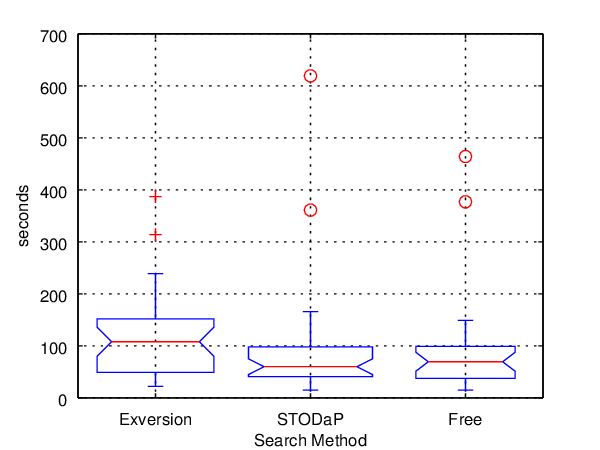
\includegraphics[scale=1.2]{images/tct_boxplotresults.png}
\caption[Boxplot for TCT.]{Boxplot for TCT. Figure shows, for each search method: median, in red; the first and third quartiles, as the bottom and top of the box, resp.; the lowest sample within 1.5 interquartile range (IQR) of the lower quartile, as the lower whisker; the highest sample within 1.5 IQR of the upper quartile, as the upper whisker; outliers between 1.5 and 3 IQR, as + (plus); and outliers higher than 3 IQR, as o (circle).}
\label{fig:tct}
\end{center}
\end{figure}

\begin{figure}[h]
\begin{center}
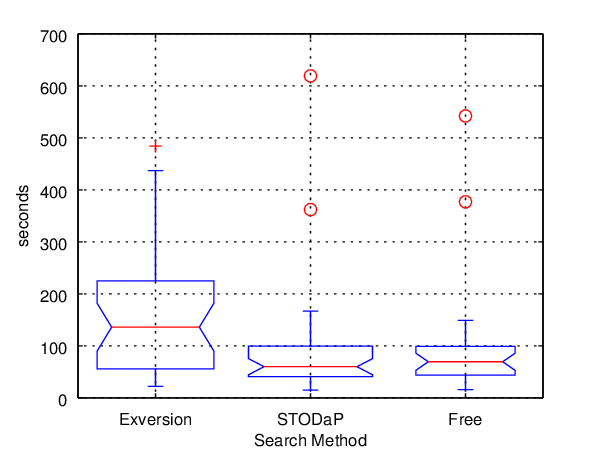
\includegraphics[scale=1.2]{images/tct_boxplotresults_notnull.png}
\caption[Boxplot for TCT$_{nb}$.]{Boxplot for TCT$_{nb}$. Elements of the plot are described in \autoref{fig:tct}.}
\label{fig:tct_nb}
\end{center}
\end{figure}

\begin{figure}[h]
\begin{center}
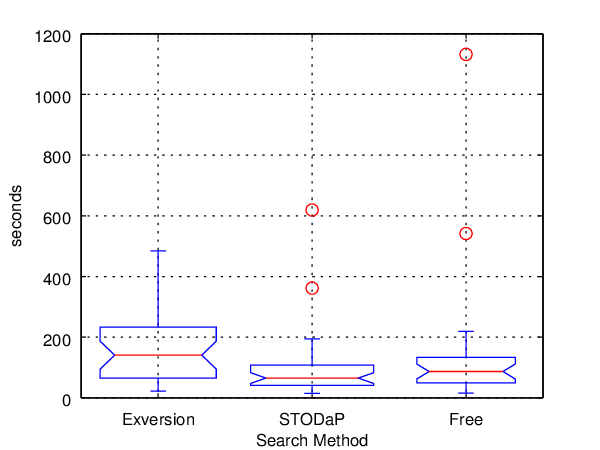
\includegraphics[scale=1.2]{images/tct_boxplotresults_correct.png}
\caption[Boxplot for TCT$_{c}$.]{Boxplot for TCT$_{c}$. Elements of the plot are described in \autoref{fig:tct}.}
\label{fig:tct_c}
\end{center}
\end{figure}



\subsection{Precision Analysis}

\autoref{fig:precision} presents an analysis of the answer precision for each search method and task.
As stated before, each answer given by participants was validated against the specified task.
Thus, we were able to compute the precision of each task as:

\begin{equation}
	P = \frac{a_v}{A_T} * 100,
\end{equation}

where $A_T$ is the number of required answers for each task, and $a_v$ is the number of valid answer given by a subject.

\begin{figure}[h!]
\begin{center}
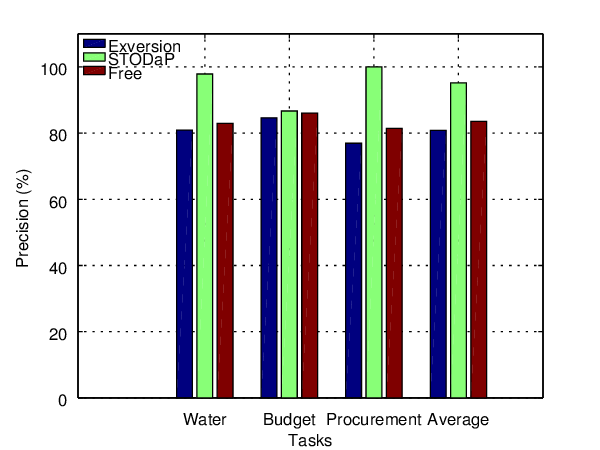
\includegraphics[width=\columnwidth]{images/precision.png}
\caption[Precision analysis.]{Precision analysis. Bars show the average precision for subjects answers, for each question and for each search method.}
\label{fig:precision}
\end{center}
\end{figure}

A parallel behaviour as in TCT analysis can be observed.
STODaP exhibits a better performance on average, but is slightly worse regarding the Budget task.
A 100\% rate can be observed in the STODaP performance for the Procurement task.
In this case, where the task required datasets in three different languages, semantic tag Public Procurement (\url{http://stodap.org/semantictag/4321/}) could directly connect datasets in English, Russian, Spanish, Finish, Portuguese, Danish, German and Italian using the keyword ``procurement''.
Thus, this task presents the better performance for STODaP, and also the worse using other methods.

\subsection{Subjective Evaluation}

After completing the tasks, subjects were filled an evaluation questionnaire, whose answers are systematized in \autoref{tab:subj_eval}.
The first question is aimed to gather an absolute view of subjects about the system.
The second one, in turn, evaluates STODaP in relation to another specialized open dataset search engine, and to generic web search engines.

Results are shown as an average of all user, but also segregated between non-experts, i.e., those who considered their open data ability being between 1 to 3, and experts, i.e., open data ability 4 or 5.
Global score shows an overall satisfaction with STODaP, both absolutely and in relation to other methods.
Segregated results shows non-experts more satisfied than experts.
This result was expected, since, as discussed before, experts normally need more specific datasets, and they know where to find it, or at least have some clues. 
STODaP fits more the needs of non-experts, by providing a generic starting point to find data.

\begin{table}[h]
\ABNTEXfontereduzida
\centering
\caption{STODaP evaluation - summary of subjective evaluation}
\label{tab:subj_eval}
\begin{tabular}{|m{4cm}|>{\centering}m{3cm}|>{\centering\arraybackslash}m{3cm}|>{\centering\arraybackslash}m{3cm}|}
\hline
\textbf{Question} & \textbf{Global Average} ($n=34$) & \textbf{Non-experts} ($n=25$) & \textbf{Experts} ($n=9$) \\ \hline
Absolute Satisfaction & 4.3 & 4.4 & 4.2 \\ \hline
Relative Satisfaction & 4.2 & 4.4 & 3.9\\ \hline
\end{tabular}
\end{table}

The evaluation questionnaire included also a free comment section, in order to let subjects write their impressions.
Unfortunately, only 14 subjects out of 34 wrote comments.
Comments can be categorized in the following categories:

\noindent \textbf{Design/Layout:} Six subjects complained about the user interface, both visually and in terms of usability: \emph{``The user interface is not intuitive nor pleasant. It should be further worked to help the visualization of results.''} was one the comments.
The absence of an interface for managing filter was also noticed: \emph{``When I select the option to filter by country, I couldn't see any way to remove that filter or which filters are currently applied in case there are more than one.''}

\noindent \textbf{Compliments: } Six users wrote positive comments, highlighting the ability of the system to support proposed tasks. One example is: \emph{``I did not manage to find any relevant datasets on river data quality after about 20 minutes of searching (using google). There were some available but they were for European rivers. The STDOaP is very useful and simple to use. Data is very easily discovered, and results are more relevant due to the availability of filtering.''}

\noindent \textbf{Language: } One comment was related to language barriers, specifically when search terms are not in English.
The translation of semantic tags label is referred on the future works.

\noindent \textbf{Missing data: } Two subjects noticed the absence of desired data, but one of them recognized that this could be due to a publishing failure, and not related to the STODaP system itself.

\noindent \textbf{Semantic Interpreter:} One subject noticed that \emph{``some improvement in semantic interpreter is needed.''}, but unfortunately no further details were given.


% \begin{table}[h!]
% \ABNTEXfontereduzida
% \centering
% \caption[Task Completion Time of the evaluation, in seconds.]{Task Completion Time of the evaluation, in seconds. 
% Each cell contains the number of seconds that one or more subjects took to complete the task with the correspondent search method.}
% \label{tab:eval_results_tct}
% \begin{tabular}{|>{\centering\arraybackslash}m{2.4cm}|>{\centering\arraybackslash}m{2.4cm}|>{\centering\arraybackslash}m{2.4cm}|>{\centering\arraybackslash}m{2.4cm}|>{\centering\arraybackslash}m{2.4cm}|>{\centering\arraybackslash}m{2.0cm}|}
% \hline
% \textbf{Tasks / Search Methods} & \textbf{Water Quality} & 	\textbf{Budget information}  &	\textbf{Procurement} &	\textbf{Average and Standard Deviation}  & \textbf{Accepted Answers (\%)} \\ \hline 
% \textbf{Exversion} & 122.89 &125.92 &122.82 &124.00 & 81.91 \\ \hline 
% \textbf{STODaP} & 83.91 &118.33 &89.00 &97.22 & 94.78 \\ \hline 
% \textbf{Free} & 101.44 &58.75 &184.00 &116.88 & 85.58 \\ \hline 
% \textbf{Average} & 101.45 & 106.28 & 126.18 &  & \\ \hline 
% \textbf{Acceptance} & 88.69 & 88.12 & 86.85 &  & \\ \hline
% \end{tabular}
% \end{table}

% \begin{table}[h!]
% \ABNTEXfontereduzida
% \centering
% \caption[Task Completion Time of the evaluation, in seconds.]{Task Completion Time of the evaluation, in seconds. 
% Each cell contains the number of seconds that one or more subjects took to complete the task with the correspondent search method.}
% \label{tab:eval_results_rate}
% \begin{tabular}{|>{\centering\arraybackslash}m{2.4cm}|>{\centering\arraybackslash}m{2.4cm}|>{\centering\arraybackslash}m{2.4cm}|>{\centering\arraybackslash}m{2.4cm}|>{\centering\arraybackslash}m{2.4cm}|>{\centering\arraybackslash}m{2.0cm}|}
% \hline
% \textbf{Tasks / Search Methods} & \textbf{Water Quality} & 	\textbf{Budget information}  &	\textbf{Procurement} &	\textbf{Average and Standard Deviation}  & \textbf{TCT (s)} \\ \hline 
% \textbf{Exversion} & 80.89 &88.33 &75.73 &81.91 &124.00 \\ \hline 
% \textbf{STODaP} & 97.45 &86.67 &100.00 &94.78 &97.22 \\ \hline 
% \textbf{Free} & 85.78 &90.00 &81.44 &85.58 &116.88 \\ \hline 
% \textbf{Acceptance} & 88.69 & 88.12 & 86.85 &  & \\ \hline 
% \textbf{TCT} & 101.45 & 106.28 & 126.18 &  & \\ \hline
% \end{tabular}
% \end{table}


% \begin{itemize}
% 	\item Task completion time for each search method (and variance) \cite{Xu2009}
% 	\item Task completion time for each task (and variance) \cite{Xu2009}
% 	\item Correlation between satisfaction and completion time for STODaP server \cite{Xu2009}
% 	\item Correlation between results found in the different search methods \cite{Vaughan2004}
% \end{itemize}

\subsection{Correlation Analysis}

In order to check the correlation between characteristics of the subjects, their evaluation of the tool and their performance on the tests we calculate the correlation coefficient between every variable related to the subjects, i.e.: (i) profile variables such as age, English proficiency, and internet, data and open data abilities; (ii) evaluation about the tool, i.e.: absolute and relative satisfaction; and (iii) test performance, i.e.: total tasks completion time and precision.

\autoref{tab:correlations} shows the results.
Age is measured in years. The six following columns are variables that scale from 1 to 5, where 1 worse option, and 5 the better.
Task Completion Time is the sum of time, in seconds, taken to complete all 3 tasks, and the last column is related to the percentage of correct answers.
As before, for this analysis, we considered only subjects with more than 33\% of correct answers.

\begin{table}[t]
\ABNTEXfontereduzida
\centering
\caption[Correlation analysis of the results.]{Correlation analysis of the results.}
\label{tab:correlations}
\begin{tabular}{|>{\arraybackslash}m{1.7cm}||>{\centering\arraybackslash}m{0.8cm}|>{\centering\arraybackslash}m{1.4cm}|>{\centering\arraybackslash}m{1.2cm}|>{\centering\arraybackslash}m{1.0cm}|>{\centering\arraybackslash}m{1.0cm}||>{\centering\arraybackslash}m{1.7cm}|>{\centering\arraybackslash}m{1.6cm}||>{\centering\arraybackslash}m{1.0cm}|>{\centering\arraybackslash}m{1.5cm}|}
 \hline 
 Variables & \textbf{Age} & \textbf{Internet} &	\textbf{English} & \textbf{Data} & \textbf{Open Data} & \textbf{Absolute Satisfaction} &	\textbf{Relative Satisfaction} & \textbf{TCT} &	\textbf{Precision} \\ \hline \hline
\textbf{Age} & 1.0 	&--	& 0.18 	& 0.52 	& 0.41 	& -0.11 	& -0.42 	& -0.16 	& 0.13 	\\ \hline
\textbf{Internet} &--	&--	&--	&--	&--	&--	&--	&--	&--	\\ \hline
\textbf{English} & 0.18 	&--	& 1.0 	& 0.39 	& 0.43 	& -0.22 	& -0.31 	& 0.11 	& 0.28 	\\ \hline
\textbf{Data} & 0.52 	&--	& 0.39 	& 1.0 	& 0.45 	& -0.18 	& -0.28 	& -0.32 	& 0.41 	\\ \hline
\textbf{Open Data} & 0.41 	&--	& 0.43 	& 0.45 	& 1.0 	& -0.21 	& -0.44 	& -0.13 	& 0.15 	\\ \hline
\textbf{Absolute Satisfaction} & -0.11 	&--	& -0.22 	& -0.18 	& -0.21 	& 1.0 	& 0.56 	& 0.15 	& 0.14 	\\ \hline
\textbf{Relative Satisfaction} & -0.42 	&--	& -0.31 	& -0.28 	& -0.44 	& 0.56 	& 1.0 	& 0.15 	& 0.08 	\\ \hline
\textbf{TCT} & -0.16 	&--	& 0.11 	& -0.32 	& -0.13 	& 0.15 	& 0.15 	& 1.0 	& 0.09 	\\ \hline
\textbf{Precision} & 0.13 	&--	& 0.28 	& 0.41 	& 0.15 	& 0.14 	& 0.08 	& 0.09 	& 1.0 	\\ \hline 
\end{tabular}
\end{table}

Looking to the correlation coefficients, only a few have a module higher than 0.5, and higher values do not reveal any unexpected results.
It is possible to observe a positive correlation between absolute usefulness and relative usability.
A negative correlation between open data ability and relative usability confirms the fitness of the system for non-experts in open data.
Data ability is negatively correlated with task completion time, and positively with precision.
English proficiency may also play a positive role regarding precision.

Although some clues can be gathered looking at \autoref{tab:correlations}, an analysis of variance (ANOVA) reveals that only a few correlations have a high confidence.
The variables whose correlation confidence (p-value) is equal or than 0.05 are: age and data ability (0.001), age and usability (0.003/0.0001), English proficiency and data ability (0.042), data and open data ability (0.029/0.02), usefulness and usability (0.002/0.003).
Regarding the experiment measures -- TCT and precision -- no relevant correlation was found.

\section{Conclusions}
\label{sec:conclusion}

% After proposing an approach for semantic organization of metadata in Open Data Portals in the previous chapter, in this chapter the approach was evaluated.

Evaluation is a crucial part of every scientific work, since without testing, it is impossible to know if the system works as designed, and if it accomplishes the proposed goals.
However, designing and implementing an information system evaluation is a very complex and challenging task.
Isolating the desired variables from other environment influences is nearly impossible, mainly because of the socio-technical characteristic of information systems.
And if we try to select the ideal subjects to perform the ideal tasks, the evaluation itself can become too complex, and chances are high that it gets too distant of reality.
One can be tempted to look for simple cause-effect explanations in complex problems, i.e., involving humans and systems.
However, according to \citeonline{Morin2011}, the world is an inseparable tissue of actions, interactions, feedbacks, determination and chances, an thus it is too simplistic to think in a direct cause-effect explanation for complex systems.

Searching for open datasets is not an everyday task for the absolute majority of the population.
On the other hand, experienced data scientists already know where to find their data, and even if this data is available or not.
With those questions in mind, we designed this evaluation trying to balance specificity and generality in the choice of subjects.
We also tried to balance the specificity of the tasks, so that it would not be too general (``Find open datasets in Brazil'') but also not too specific (``Find the open data set of 2015 budget in Rio de Janeiro'').
Following this reasoning we chose our subjects (Computer Science students that could work one day with open data and Semantic Web researchers and practitioners that already work with open data), and our tasks (finding datasets on specific themes according to language and geographical limitations).

Results shows that, for the designed tasks, STODaP outperforms Exversion Data Search Engine and generic web search engines regarding time to complete tasks and precision of the answers.
It can also be concluded that STODaP performance is better when less data is available.
In cases were data availability is high, such as budget data, web search engines may find more precise data in less time.

Subjective evaluation about the system was positive, both regarding absolute usefulness, and in relation to other search methods.
Subjects with a lower open data experience tend to rate the system better than experts.
Statistical correlation analysis confirmed that subjects with a higher data manipulation ability finish their tasks faster and with a higher precision.
English proficiency seems also to play a positive role regarding precision.
However, no interesting correlation could be confirmed by a relevance test.

Comments written by subjects point out several enhancement suggestions, e.g. regarding layout and design, semantic interpretation and multi-language enhancements.
The absence of data for some topics was also noticed, recognizing this gap as a governmental transparency issue.

In the next chapter, we summarize our contributions, indicating the limits of this research and pointing out the way for continuing this work.